The architecture was built through the iterative methodology AOPOA, \todo[inline]{it is missing a reference to the AOPOA methodology} which allows the decomposition of goals in smaller goals until the desired granularity is reached. The starting point was the global agent's goal to perform a sequence of actions coherent, given a script. This section describes the final result of this methodology showing in the Figure~\ref{fig:generalArchitecture}, where is shown the four modules that compound it: configuration, action, belief, and motivation.
\begin{figure}
	\centering
	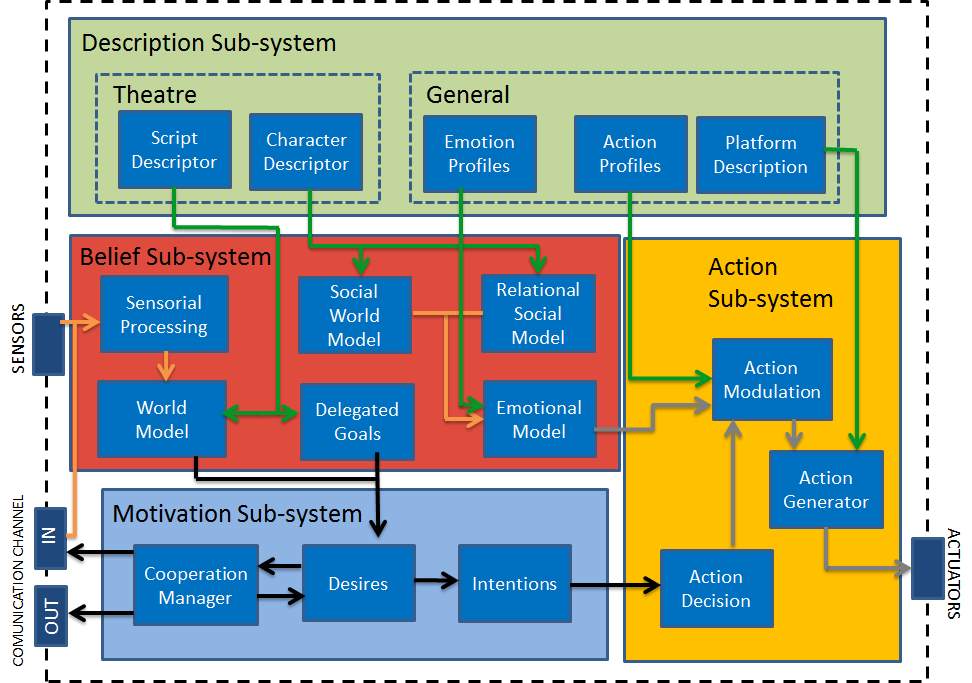
\includegraphics[width=0.5\textwidth]{Images/GeneralArchitecture.png} 
	\caption{General architecture . The green arrows show the information that comes from the configuration module about the script information and the robotic platform information. The orange arrows are information that is relevant to update the beliefs and the internal state of the agent. The black arrows represent information about the current goals that the agent wants to achieve and how this information becomes in an action. Finally, the gray arrow represent how the action is affected by the emotional state and how the action is executed in the current platform's agent.}
	\label{fig:generalArchitecture}
\end{figure}
\subsubsection{Belief Manager}
This module handles has and update the mental state of the robot-actor. This goal is achieve in two different ways: first, the perception phase collects and processes relevant information about the world, and it updates its internal model of the world.
\subsubsection{Motivation Manager}
The motivation manager is in charge of the deliberative process, in other words  this group is responsible for the big question: what should the agent do?. The design of this group has done in concordance with the belief-desired-intention model but also, incorporate a communication manager that allow the coordination between robo-actors when it is required.
\subsubsection{Action Controller}
The action controller manages all the process of action selection, and the modulation of the actions to convey emotions. This modulation is done using the agent's emotional state. In this way the emotional state does not interfere in the decision process.
\subsection{Configuration Module}
Configuration module has all the information that are necessary to perform emotional actions, and the description of the script that the robot has to follow.